\documentclass[11pt]{article} 
\usepackage{geometry} \geometry{hmargin={1in,1in},vmargin={1in,1in}} 
\usepackage{amsmath,amsfonts,amssymb,color} 
\usepackage[dvips]{graphics} 
\usepackage[dvips]{graphicx} 
\begin{document} 
\begin{center}
{\bf \Large Bubble Report} 
\end{center}
\section{Parameters:} 
This is a report that examines an immersed fiber initially expressed in terms of cosine perterbations of a circle. The initial conditions are set using:
\begin{equation} 
 r = R + A \cos( n\theta) \label{bubble}
\end{equation} 


 \vskip.2in \noindent This code was run on 3/23/2010 with the parameters given in the following table:
 \begin{table}[!htp] 
\begin{center} 
\vskip.1in 
\begin{tabular}{|l|l|l|l|l|} \hline 
Grid: &  Time: & Fluid: & IB: & Bubble: \\  \hline \hline 
$[x_{min} , x_{max}] $ =  [-2.5,2.5] & $T$= 1.0 & $Re$ = 100.0& npts = 349& $R $ = 1.0\\ 
$[y_{min} , y_{max}] $ =  [-2.5,2.5] & $N$= 250& $\lambda$ = 0.0 & $\sigma$ = 100.0& $A$ = 0.2\\ 
$(x_{pts},y_{pts})$    =  (128,128) & $\mbox{total}_{\mbox{saves}}$ = 5 & $\alpha$ = 0.0 & & $n$ = 3.0\\ 
& $\Delta t$ = 0.004& $\epsilon$ = 0.0 & & \\ 
&  & $\nu$ = 0.0 &  & \\ \hline 
 \end{tabular} 
\caption{Numerical Model Parameters} 
\end{center}
\label{parameters} 
\end{table} 

 \noindent The Giesekus constitutive model for viscoelastic fluid flow was used: 
\newcommand{\bu}{\mbox{\boldmath $u$}}\newcommand{\bs}{\mbox{\boldmath ${\sigma}$}}\begin{eqnarray*}
 \bs + \lambda \left( {\color{black}\frac{\partial  \bs}{\partial t }}+ \bu \cdot \nabla \bs -(\nabla\bu) \bs - \bs(\nabla\bu)^T - \nu\Delta \bs + \epsilon \bs^2  \right) - 2\alpha {\bf d}(\bu) & = & 0 \;\; \mbox{in } \Omega \\ 
Re\left({\color{black}\frac{\partial \bu}{\partial t}} + \bu\cdot\nabla \bu\right) + \nabla p - 2(1-\alpha)\nabla \cdot {\bf d}(\bu) - \nabla \cdot \bs & = & {\bf f} + {\bf F_{IB}} \;\; \mbox{in } \Omega \\ 
\nabla \cdot \bu & = & 0  \;\; \text{in} \;\; \Omega 
\end{eqnarray*} 

\section{Immersed boundary forces:}
The Forces are set based on the curvature of the immersed fiber. With the curve defined in polar coordinates  as $ r(\theta)$ the forces at point $\theta$ on the fiber are: 
\[ F(\theta) = \sigma \kappa(\theta) {\bf n}  \]
 where 
 \[ \kappa(\theta) = \frac{(r^2 + 2(r')^2 - r r'')}{\left((r)^2 + (r')^2 \right)^{\frac{3}{2}}} \]
 is the curvature of the fiber, ${\bf n}$ is the outward normal and $\sigma$ is a material parameter. The values of $r, r'$ and $r''$ are the radius, and its derivates with respect to $\theta$.\section{Plot of immersed boundary: }

 A plot of the immersed boundary at time $t=0$ and $t = 1.0$ is given in Figure \ref{Fig:FirstAndLast}.\begin{figure}[h] 
\begin{center} 
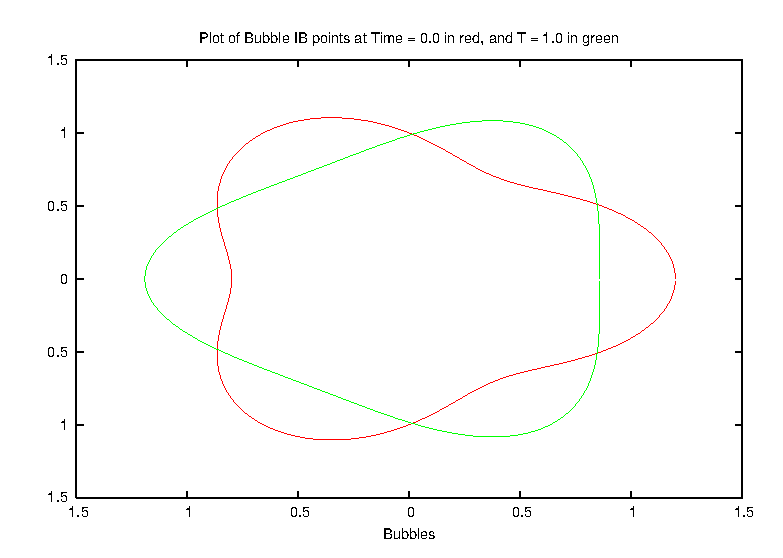
\includegraphics[width=2.65in, height=2.65in, angle=0]{FirstAndLastIBPoints3} \\ 
\caption{Plot of immersed boundary at $t = 0$ and $t = 1.0$. \label{Fig:FirstAndLast}} 
\end{center} 
\end{figure} 
\section{Plot of FFT Modes: }

 Equally distributing a set of points about the fiber with respect to $\theta$, the amplitude of the 3 mode is tracked and plotted vs. time and shown as a red line in Figure \ref{Fig:FFTModep}.\begin{figure}[h] 
\begin{center} 
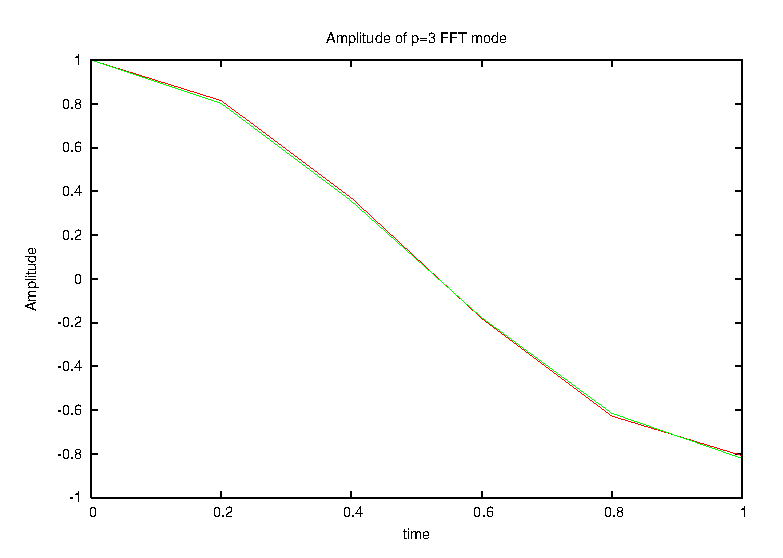
\includegraphics[width=6in, height=2in, angle=0]{AmpModePlot3.eps} \\ 
\caption{Plot of the FFT of mode 3. \label{Fig:FFTModep}} 
\end{center} 
\end{figure} 
The best fit parameters $d_r$ and $\omega$ are found to fit the tracted FFT mode such that 
\[ y = e^{(-d_r t)} \cos(\omega t). \]
 Specifically the code found 
 \[ d_r = 0.178179309724 \hskip0.5in \mbox{and } \hskip0.5in \omega = 2.94785733523.\] 
 The best fit function is plotted as a green line in Figure \ref{Fig:FFTModep}. A plot of a second excited mode is also tracked and plotted. Specifically the 6 mode is shown in Figure \ref{Fig:FFT2Modep}. \begin{figure}[h] 
\begin{center} 
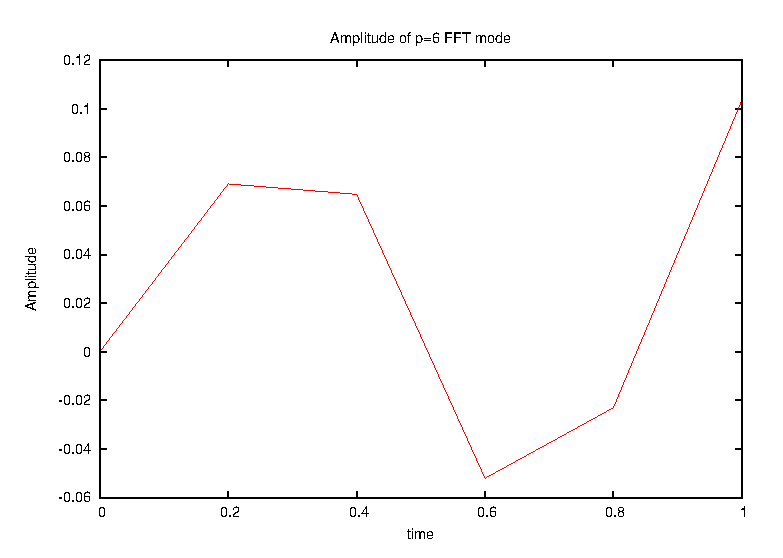
\includegraphics[width=6in, height=2in, angle=0]{Amp2ModePlot3.eps } \\ 
\caption{Plot of the FFT of mode 6. \label{Fig:FFT2Modep}} 
\end{center} 
\end{figure} 
\section{Report Location:} 


This report was generated using the data located in: \\ 
{\footnotesize 
 \verb' ./RunOn3_23_2010Bree/ '}
\end{document} 
